
%----------------------------------------------------------------------------------------
%	PACKAGES AND OTHER DOCUMENT CONFIGURATIONS
%----------------------------------------------------------------------------------------

\documentclass[12pt]{article}
\usepackage[english]{babel}
\usepackage{amsmath}
\usepackage{graphicx}
\usepackage{float}
\usepackage[colorlinks = true,
linkcolor = blue,
urlcolor  = blue,
citecolor = blue,
anchorcolor = blue]{hyperref}
\usepackage{blindtext}


\begin{document}
	
	\begin{titlepage}
		
		\newcommand{\HRule}{\rule{\linewidth}{0.5mm}} 
		
		\center % Center everything on the page
		
		%----------------------------------------------------------------------------------------
		%	HEADING SECTIONS
		%----------------------------------------------------------------------------------------
		\textsc{\Large MSc Project: Mobile Hairdresser Application}\\[5 cm] 

		
		
		
\includegraphics[scale=0.05]{images/logo.png}\\[1 cm]
				
		

		
		
		\textsc{\LARGE Joshua Robertson} \\[6 cm]
		
		

		
		
		%----------------------------------------------------------------------------------------
		%	TITLE SECTION
		%----------------------------------------------------------------------------------------
		
		
		
		%----------------------------------------------------------------------------------------
		%	AUTHOR SECTION
		%----------------------------------------------------------------------------------------
		
		
		\begin{center}
			
			\textsc\emph{{“A dissertation submitted to the University of Bristol in accordance with the requirements of the degree of Master of Science by advanced study in Computer Science in the Faculty of Engineering."}} \\[1.2 cm]
			
			School of Computer Science, Electrical and Electronic Engineering, and Engineering Maths (SCEEM) \\[1 cm]
			
			
			
		\end{center}
		
		
		
		
		\vfill % Fill the rest of the page with whitespace
		
	\end{titlepage}
	
	\section{Introduction}
	The COVID pandemic has brought with it a shift in perceptions around leaving the home and with that a desire for more homeworking and access to remote services. For example, remote workers show an increase in job satisfaction \cite{flexjobs, 2019}, \cite{CNBC, 2020}, are more productive, have better mental health \cite(flexjobs, 2020) and even make more money (ADD CITE).
	
	New Product Development refers to the entirety of processes leading to bringing a product to market and encompasses several steps as seen in figure \ref{fig:npd} below.
	\newline
	
	\begin{figure}[H]
		\centering
		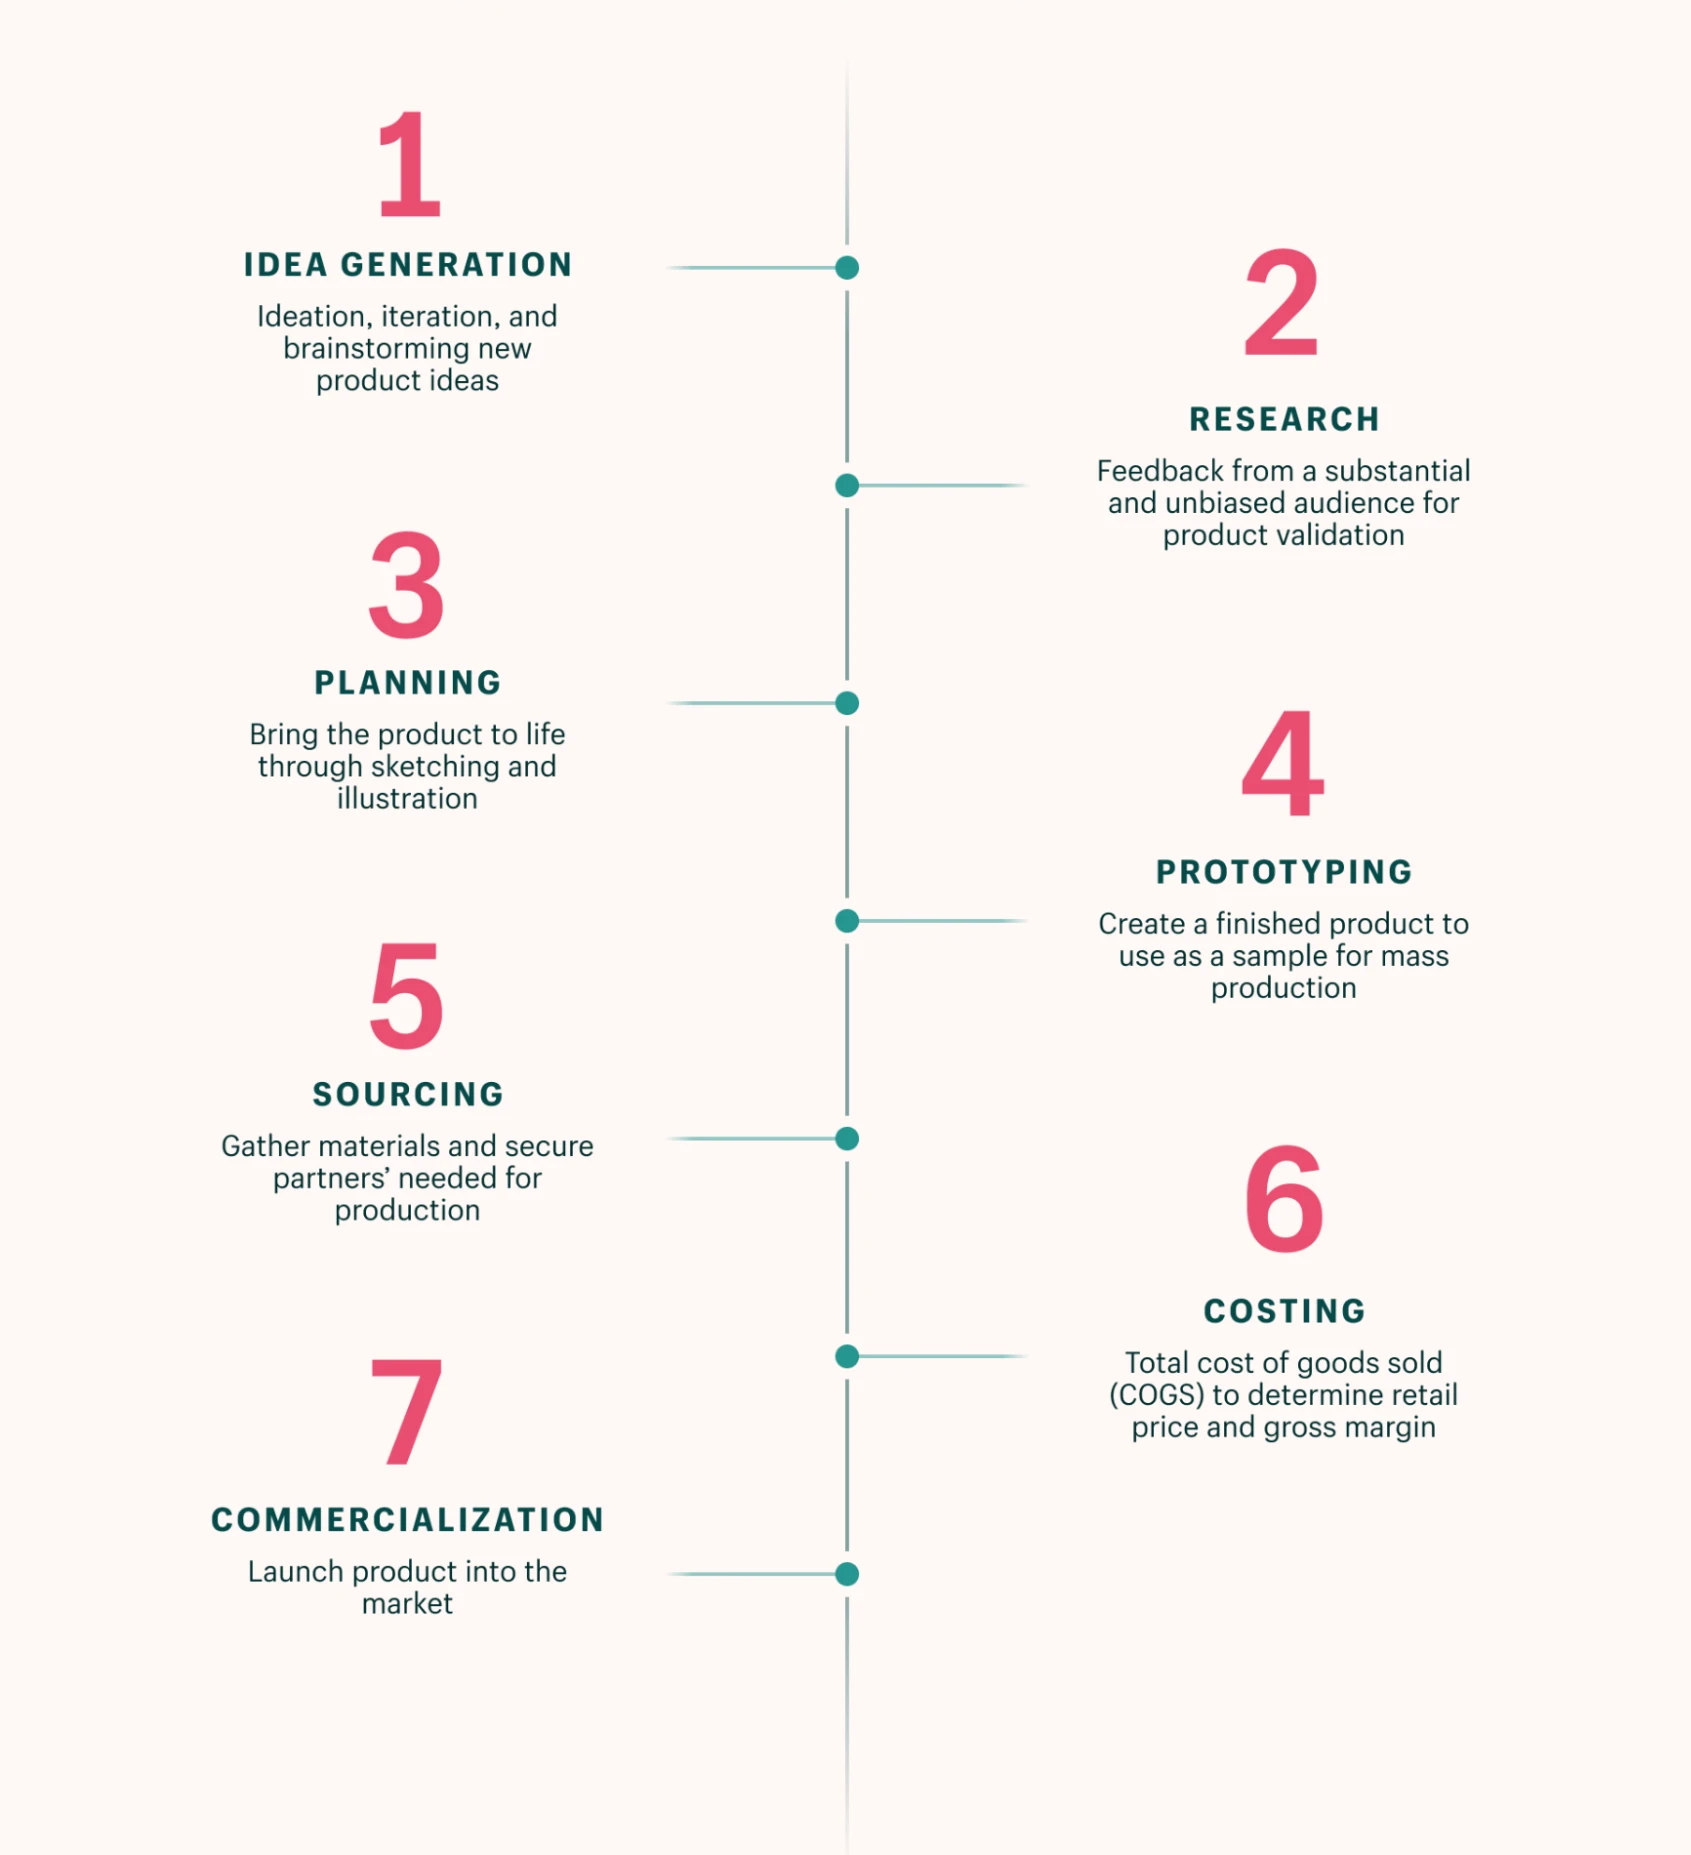
\includegraphics[scale=0.15]{images/npd.png}
		\caption{The 7 Steps of New Product Development}
		\label{fig:npd} \cite{shopify}
	\end{figure}
	
	
	\subsection{Ideation and Concept}
	\blindtext
	
	\subsection{Market Analysis}
	In order to gauge whether there is a market for the proposed analysis, a survey was carried out in which users were asked about whether they could see themselves using the application features, among other things.
	 
	\subsubsection{Existing Applications}
	
	\subsection{Deciding on a Platform}
	\subsubsection{Mobile vs Desktop}
	
	\subsubsection{Android vs iOS}
	An important consideration when creating a mobile application is deciding on which platform to choose. The two largest mobile providers currently are android and apple (iOS). Historically, iOS has dominated the market share, with a 42.02\% market share in January 2011 compared to Androids 12.42\% (figure \ref{fig:ios-android}). Despite this, in recent years android OS has become more popular, even holding a greater share several times over the last few years and currently trails by only around 2\%.
	
	\begin{figure}[H]
		\centering
		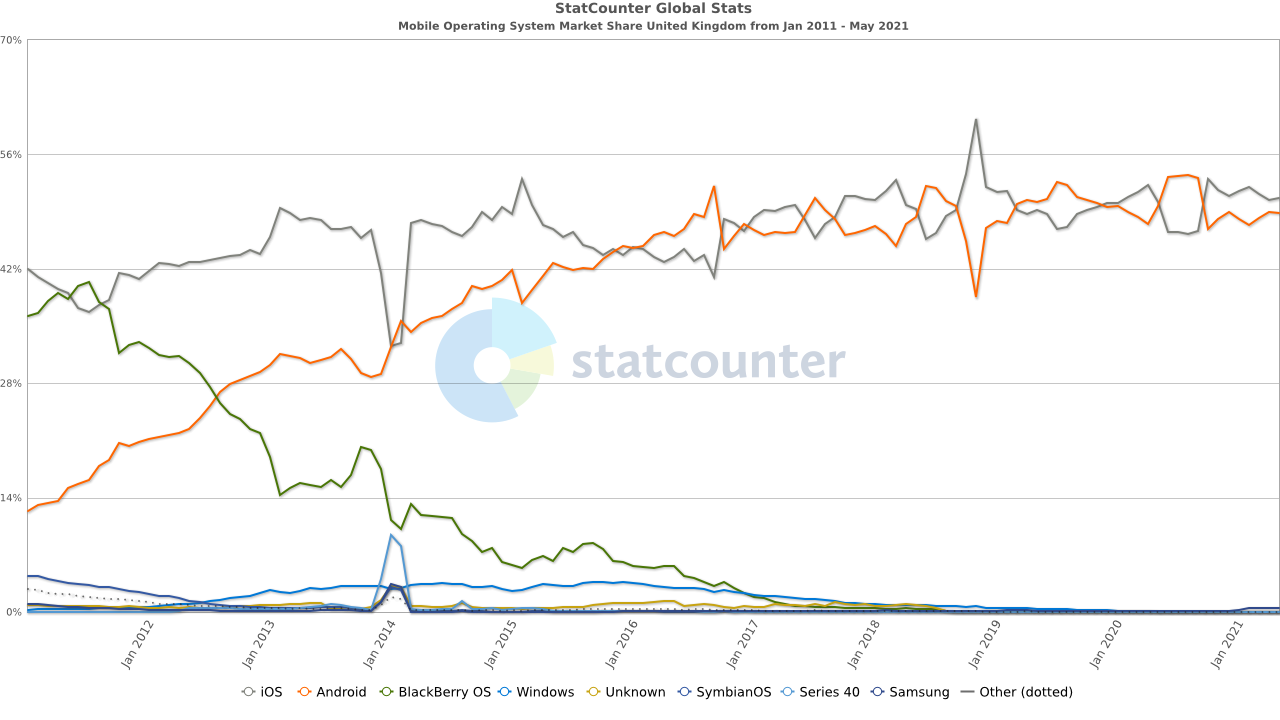
\includegraphics[scale=0.4]{images/ios-android.png}
		\caption{iOS vs Android Market Share Over The Last 10 Years}
		\label{fig:ios-android}
		\cite{stat-counter-21}
	\end{figure}
	
	With this change has brought with it a push towards frameworks that allow for development across multiple platforms, such as React Native (https://reactnative.dev/) and Flutter (flutter.dev/). For this reason, a cross platform application using Flutter as the development framework was used to create the application. In this way, both operating systems can be targeted and the application can be accessed by the greatest number of users.
	
	
	\subsubsection{The Target User}
	
	\subsubsection{Programming Language}
	When deciding on the programming software, several metrics were taken into consideration, including cross-platform functionality, speed, speed of development and performance. For this reason, Dart and the corresponding Flutter software development kit (SDK) were chosen for the primary software. Flutter is a cross-platform development kit, meaning that it will natively run on both iOS and android applications created by Google \cite{flutter}. Dart is compiled ahead-of-time into native ARM code giving better performance compared to other similar development kits, such as React Native and the user interface  is implemented within a fast, low-level C++ library giving great speed to the application. Dart has also seen a large increase in usage within recent years, jumping up 532\% from 2018 to 2019 \cite{Github, 2018} meaning that there is now an extensible list of third-party plugins available and a large community.
	

	\subsection{User Personas}
	The creation of user personas representing fictitious, archetypal users is an essential part of application development \cite{Grudin and Pruitt, 2002} and allows a deep understanding of the target user to be sought and implemented within the features and design of the application \cite{Long, 2009}. There are, however some shortcomings to qualitative persona generation, such as validity concerns and user bias \cite{Chapman and Milham, 2007} and although they are addressed by other methods, such as data-driven personas \cite{Mcginn and Kotamraju, 2008}, there require a broad user base and therefore we have decided to stick with qualitative methods, which allow for enough brevity and depth for the scope of the project. Here we created 3 personas, which are discussed in detail below.
	\begin{itemize}
		\item Persona 1: 
		
		INSERT PERSONA INFO
		\item Persona 2:
		\item Persona 3:
	\end{itemize}

	\section{Prototyping}
	An important component of UCD and more generally UX is wireframing, which involves making a mock-up of the application that acts as an early prototype to influence later development, along with allowing for early beta testing \cite{Arnowitz Arent Berger}. For the wireframing application Adobe XD was chosen for several reasons. Firstly, it has strong prototyping functionality, allowing the user to click around the application through the use of ‘components’. This interactivity means that early testers can get a real feel for how the application works. An illustration of this can be seen below, whereby each arrow represents a state change in the form of a trigger/ action pair, whereby for example a user could click on ‘Available Right Now’ and be taken to the ‘Checkout’ as seen in figure \ref{fig:prot-comp} below.
		\begin{figure}[H]
		\centering
		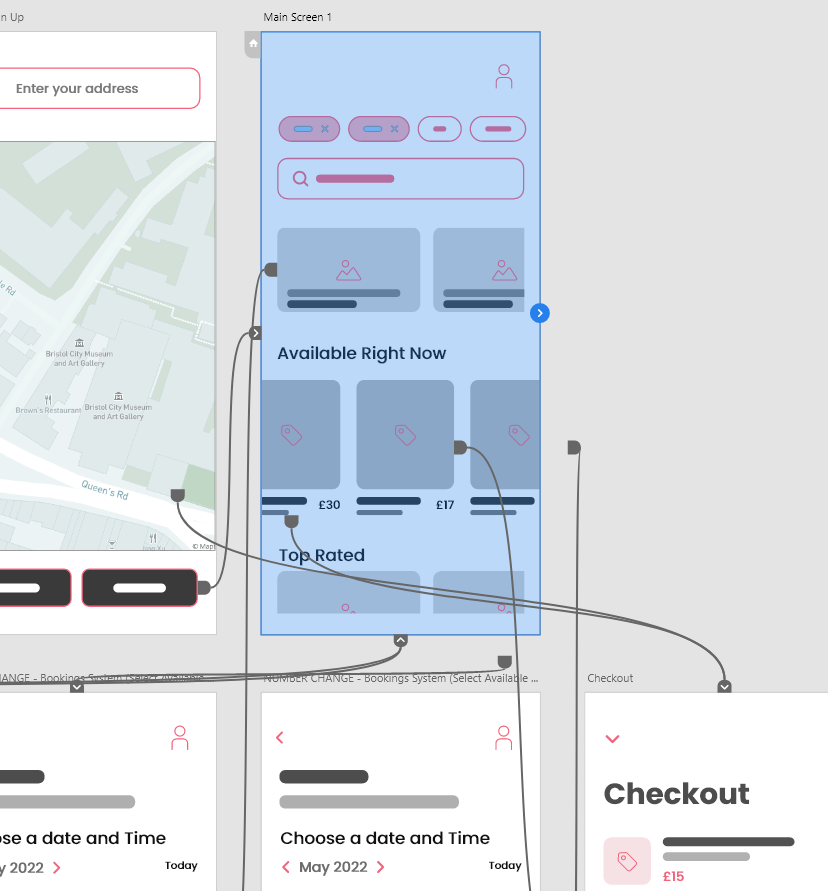
\includegraphics[scale=0.5]{images/prototyping-components.png}
		\caption{Component Interactivity within Adobe XD}
		\label{fig:prot-comp}
	\end{figure}
	
	
	Adobe XD also allows for easy distribution of the prototype in the form of a sharable link that opens in the browser and encompasses the same functionality and components that can be found within the application itself, meaning that anyone with access to a browser can test the prototype. Along with this, this prototype also allows for comments to be made, which are fed back to the owner. This comment capability was used early on during beta testing when it was sent out with the early questionnaire and influenced initial design decisions \cite{smashing-magazine}.
	
	When designing the screens there was a strong focus on user experience following Nielsons 10 Heuristics for User Interface Design \cite{nielson-normal-group-2020} . For example, the functionality was kept as minimal as possible to avoid clittering and avoid cognitive load on the user, the user was given control to go back to previous screens to allow for user control and freedom and simple and self-explanatory language was used to apply recognition over recall. For example, the Sign In screen below extraneous text was kept to a minimum by using images for the login items, such as Google, Facebook and Twitter, a sign up button was included to allow the user to access the application through creating a new account and large, clear sign in forms and buttons were used.
	
	\begin{figure}[H]
		\centering
		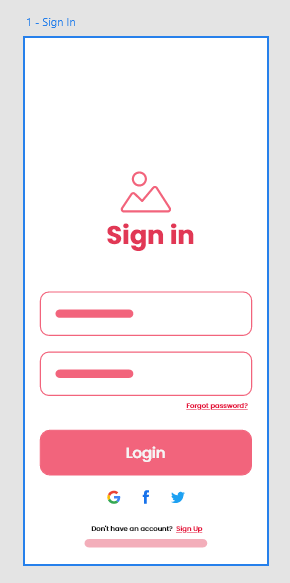
\includegraphics[scale=0.85]{images/sign-in.png}
		\caption{Sign In Page Made with Adobe XD}
		\label{fig:sign-in}
	\end{figure}
	
	\section{Production}
	\subsection{Version Control}
	
	\subsection{Sprint 1 - Setup}
	During the first sprint, the task involved setting up the environment in preparation to begin development. For the editor, Android Studio was 
	
	\subsection{Sprint X - UI}
	Flutter offer an Adobe XD plugin to turn wireframes directly into code, however, this was not used for several reasons. In Adobe XD components are positioned absolutely, whereas in Flutter it is done relatively, leading to several issues with positioning. Adobe XD also does not contain customer properties and therefore mapping these to components, such as title is not possile.
	

	
\end{document}